%%%%%%%%%%%%%%%%%%%%%%%%%%%%%%%%%%%%%%%%%
% a0poster Portrait Poster
% LaTeX Template
% Version 1.0 (22/06/13)
%
% The a0poster class was created by:
% Gerlinde Kettl and Matthias Weiser (tex@kettl.de)
% 
% This template has been downloaded from:
% http://www.LaTeXTemplates.com
%
% License:
% CC BY-NC-SA 3.0 (http://creativecommons.org/licenses/by-nc-sa/3.0/)
%
%%%%%%%%%%%%%%%%%%%%%%%%%%%%%%%%%%%%%%%%%

%----------------------------------------------------------------------------------------
%	PACKAGES AND OTHER DOCUMENT CONFIGURATIONS
%----------------------------------------------------------------------------------------

\documentclass[a0,portrait]{a0poster}

% increase some sizes
\renewcommand{\footnotesize}{\fontsize{20.74}{25}\selectfont}
\renewcommand{\small}{\fontsize{24.88}{30}\selectfont}
\renewcommand{\normalsize}{\fontsize{29.86}{37}\selectfont}

\usepackage{algpseudocode}
\usepackage{algorithm}
\usepackage{multicol} % This is so we can have multiple columns of text side-by-side
\columnsep=100pt % This is the amount of white space between the columns in the poster
\columnseprule=1pt % This is the thickness of the black line between the columns in the poster

\usepackage[svgnames]{xcolor} % Specify colors by their 'svgnames', for a full list of all colors available see here: http://www.latextemplates.com/svgnames-colors

% \usepackage{tikz}
\usepackage{pgfplots}
% options for pgfplots
\pgfplotsset{compat=1.8,compat/show suggested version=false}
\usetikzlibrary{calc,trees,arrows,patterns,plotmarks,shapes,snakes,er,3d,automata,backgrounds,topaths,decorations.pathmorphing,decorations.markings}
%\pgfplotsset{compat=newest}
\pgfplotsset{
   /pgfplots/bar  cycle  list/.style={/pgfplots/cycle  list={%
        {black,fill=black!30!white,mark=none},%
        {black,fill=red!30!white,mark=none},%
        {black,fill=green!30!white,mark=none},%
        {black,fill=yellow!30!white,mark=none},%
        {black,fill=brown!30!white,mark=none},%
     }
   },
}
% begin of externalization
\usetikzlibrary{external}
\tikzexternalize[prefix=out/]
\tikzexternalize
% don't externalize todonotes
%\makeatletter
%\renewcommand{\todo}[2][]{\tikzexternaldisable\@todo[#1]{#2}\tikzexternalenable}
%\makeatother
% end of externalization
\usetikzlibrary{patterns}
\usepgfplotslibrary{groupplots}
\pgfplotsset{
every axis label/.append style={font=\normalsize},
tick label style={font=\small},
}
\usepackage{times} % Use the times font
%\usepackage{palatino} % Uncomment to use the Palatino font

\usepackage{graphicx} % Required for including images
%\graphicspath{{figures/}} % Location of the graphics files
\usepackage{booktabs} % Top and bottom rules for table
\usepackage[font=normalsize,labelfont=bf]{caption} % Required for specifying captions to tables and figures
\usepackage{amsfonts, amsmath, amsthm, amssymb} % For math fonts, symbols and environments
\usepackage{wrapfig} % Allows wrapping text around tables and figures
\usepackage{subcaption}

\definecolor{mygreen}{rgb}{0,0.6,0}
\definecolor{mygray}{rgb}{0.5,0.5,0.5}
\definecolor{mymauve}{rgb}{0.58,0,0.82}
\usepackage{listings}
\lstset{ %
  backgroundcolor=\color{white},   % choose the background color; you must add \usepackage{color} or \usepackage{xcolor}
  basicstyle=\ttfamily, % the size of the fonts that are used for the code
  breakatwhitespace=false,         % sets if automatic breaks should only happen at whitespace
  breaklines=true,                 % sets automatic line breaking
  captionpos=b,                    % sets the caption-position to bottom
  commentstyle=\color{mygreen},    % comment style
  deletekeywords={...},            % if you want to delete keywords from the given language
  escapeinside={\%*}{*)},          % if you want to add LaTeX within your code
  extendedchars=true,              % lets you use non-ASCII characters; for 8-bits encodings only, does not work with UTF-8
  frame=leftline,                  % adds a frame around the code
  keepspaces=true,                 % keeps spaces in text, useful for keeping indentation of code (possibly needs columns=flexible)
  keywordstyle=\color{blue},       % keyword style
  morekeywords={*,...},            % if you want to add more keywords to the set
  numbers=left,                    % where to put the line-numbers; possible values are (none, left, right)
  numbersep=10pt,                   % how far the line-numbers are from the code
  numberstyle=\small\color{mygray}, % the style that is used for the line-numbers
  rulecolor=\color{black},         % if not set, the frame-color may be changed on line-breaks within not-black text (e.g. comments (green here))
  showspaces=false,                % show spaces everywhere adding particular underscores; it overrides 'showstringspaces'
  showstringspaces=false,          % underline spaces within strings only
  showtabs=false,                  % show tabs within strings adding particular underscores
  stepnumber=1,                    % the step between two line-numbers. If it's 1, each line will be numbered
  stringstyle=\color{black},     % string literal style
  tabsize=1,                       % sets default tabsize to 2 spaces
  title=\lstname                   % show the filename of files included with \lstinputlisting; also try caption instead of title
}

% some useful shortcuts
\newcommand{\ie}{\textit{i.e., }}
\newcommand{\eg}{\textit{e.g., }}
\newcommand{\etal}{et al.\ }
\newcommand{\CC}{C\nolinebreak\hspace{-.05em}\raisebox{.5ex}{\tiny\bf +}\nolinebreak\hspace{-.10em}\raisebox{.5ex}{\tiny\bf +}}

% units for results
\newcommand{\uj}{\,$\mu$J}
\newcommand{\mw}{\,mW}
\newcommand{\uw}{\,$\mu$W}
\newcommand{\ns}{\,ns}
\newcommand{\us}{\,$\mu$s}
\newcommand{\ms}{\,ms}
\newcommand{\KB}{\,KB}
\newcommand{\MB}{\,MB}
\newcommand{\GB}{\,GB}
\newcommand{\MHz}{\,MHz}
\newcommand{\GHz}{\,GHz}

% \newcommand{\SYSTEM}{Bard}
% \newcommand{\system}{bard}
% new latex commands:
%   Remove long section
\newcommand{\PUNT}[1]{}

%   Referencing various pieces of the document:
\newcommand{\figref}[1]{Figure~\ref{fig:#1}}
\newcommand{\figsref}[2]{Figures~\ref{fig:#1} and~\ref{fig:#2}}
\newcommand{\figrref}[2]{Figures~\ref{fig:#1}--\ref{fig:#2}}
\newcommand{\secref}[1]{Section~\ref{sec:#1}}
\newcommand{\secsref}[2]{Sections~\ref{sec:#1} and~\ref{sec:#2}}
\newcommand{\eqnref}[1]{Eqn.~\ref{eqn:#1}}
\newcommand{\eqnsref}[2]{Eqns.~\ref{eqn:#1} and~\ref{eqn:#2}}
\newcommand{\eqnrref}[2]{Eqns.~\ref{eqn:#1}--\ref{eqn:#2}}
\newcommand{\insref}[1]{Instruction~\ref{ins:#1}}
\newcommand{\tblref}[1]{Table~\ref{tbl:#1}}
\newcommand{\appref}[1]{Appendix~\ref{app:#1}}
\newcommand{\algoref}[1]{Algorithm~\ref{algo:#1}}

\newcommand{\argmin}{\arg\!\min}
\newcommand{\argmax}{\arg\!\max}
\newcommand{\minimize}{minimize}
\newcommand{\optimize}{optimize}
\newcommand{\st}{s.t.}

\newcommand{\app}[1]{\mbox{\texttt{#1}}}
\newcommand{\interface}[1]{\textbf{#1}}
\newcommand{\function}[1]{\mbox{\texttt{#1}}}
\newcommand{\struct}[1]{\emph{#1}}
\newcommand{\variable}[1]{\emph{#1}}
\newcommand{\pc}[1]{\mbox{\texttt{#1}}}

\newcommand{\PAD}{\vskip 0.75cm}

\usepackage[natbib=true,backend=bibtex,firstinits=true,style=numeric-comp,sorting=nyt,defernumbers,maxnames=2,maxcitenames=2,doi=false,isbn=false,url=false]{biblatex}
\bibliography{seec}

% Use bold for vectors instead of arrows
\renewcommand{\vec}[1]{\mathbf{#1}}

% Because the default settings for a0poster leave way too much whitespace!
\setlength{\topmargin}{3 cm}
\setlength{\oddsidemargin}{3 cm}
\addtolength{\textwidth}{3cm}
\addtolength{\textheight}{4cm}

\begin{document}

%----------------------------------------------------------------------------------------
%	POSTER HEADER 
%----------------------------------------------------------------------------------------

\begin{minipage}[b]{\linewidth}
\begin{center}

\includegraphics[height=5cm]{figures/uchicago_logo.png} %[width=20cm]
\hspace{18cm}

\includegraphics[height=5cm]{figures/lbnl_logo.png}
\hspace{18cm}

\includegraphics[height=5cm]{figures/ceres-logo.png}\\
\vspace{0.25cm}
\noindent\makebox[\linewidth]{\rule{0.9\paperwidth}{0.4pt}}
\vspace{0.25cm}
\end{center}

\Huge \color{NavyBlue} \textbf{Energy Efficient Application Resource Scheduling using ML Classifiers} \color{Black}\\[0.5cm] % Title
% \veryHuge \color{NavyBlue} \textbf{Bard} \color{Black}\\[0.5cm] % Title
% \Huge\textit{A Unified Framework for Managing Soft Timing and Power Constraints}\\[1.5cm] % Subtitle
%\begin{center}
\huge \textbf{Connor Imes, Steven Hofmeyr$^*$, and Henry Hoffmann}\\[0.25cm] % Author(s)
\LARGE \textbf{University of Chicago, Lawrence Berkeley National Laboratory$^*$}\\ % University/organization
\Large \textbf{ckimes@cs.uchicago.edu, shofmeyr@lbl.gov, hankhoffmann@cs.uchicago.edu}
% \\
%\end{center}
\end{minipage}
%

%\vspace{1cm} % A bit of extra whitespace between the header and poster content

%----------------------------------------------------------------------------------------

\begin{multicols}{2} % This is how many columns your poster will be broken into, a portrait poster is generally split into 2 columns

%----------------------------------------------------------------------------------------
%	ABSTRACT
%----------------------------------------------------------------------------------------

\color{Navy} % Navy color for the abstract

\begin{abstract}

% \small
\normalsize
Performance and power management in High Performance Computing (HPC) has historically favored a \emph{race-to-idle} approach in order to complete applications as quickly as possible, but this is not energy-efficient on modern systems.
As we move toward exascale and hardware over-provisioning, power management is becoming more critical than ever for HPC system administrators, opening the door for more balanced approaches to performance and power management.
We propose maximizing \emph{energy efficiency} to achieve an optimal balance of performance and energy consumption, eventually even increasing the throughput of over-provisioned clusters.

\end{abstract}

%----------------------------------------------------------------------------------------
%	INTRODUCTION
%----------------------------------------------------------------------------------------

%\color{SaddleBrown} % SaddleBrown color for the introduction

%\section*{Introduction}

%----------------------------------------------------------------------------------------
%	OBJECTIVES
%----------------------------------------------------------------------------------------

\color{DarkSlateGray} % DarkSlateGray color for the rest of the content

% \vspace{-1cm}
% \section*{Motivation}


%----------------------------------------------------------------------------------------
%	MATERIALS AND METHODS
%----------------------------------------------------------------------------------------

% \vspace{-1.5cm}
\section*{Intro and Design}

Tuning \textbf{core allocation (taskset)} and \textbf{dynamic voltage and frequency scaling (DVFS)} can save energy by power-gating unneeded cores and scaling back active processors, \eg during I/O or for code not on the critical path.
Both are available in HPC job schedulers, though unfortunately today they are typically only configurable when a job is launched.

{
\PAD
\PAD
\centering
  \tikzset{%
  app/.style    = {draw, thin, rectangle, minimum height = 2.5em,
    minimum width = 5em, fill=black!25},
  block/.style    = {draw, thick, rectangle, minimum height = 3em,
    minimum width = 5em},
  blockres/.style    = {draw, thick, rectangle, minimum height = 3em,
    minimum width = 5em, fill=green!25},
  biblock/.style  = {draw, thick, rectangle, minimum height = 6em,
    minimum width = 6em, fill=red!25},
  sum/.style      = {draw, circle, node distance = 4cm}, % Adder
  input/.style    = {coordinate}, % Input
  output/.style   = {coordinate} % Output
}

\begin{tikzpicture}[scale=1.0,transform shape, auto, thick, node distance=1.5cm, >=triangle 45]

\draw
  % Drawing the top blocks
  % node [input, name=goalaccuracy] {} 
  % node [left of=goalaccuracy, node distance=0.35mm]{}
  % node [sum, right of=goalaccuracy] (sumaccuracy) {} % negative feedback
  node [block, align=center] (featureselection) 
    {Feature\\Selection}
  node [block, right of=featureselection, align=center, node distance=12cm] (classifier) 
    {Classifier}
  node [blockres, above of=classifier, align=center, node distance=5cm] (trainingdata) 
    {Training\\Data}
;
  % Connectng lines
% \draw[->](goalaccuracy) -- node[align=center] {Timing\\Goal}(sumaccuracy);
% \draw[->](sumaccuracy) -- node[align=center] {Timing\\Error}(featureselection);
\draw[->](featureselection) -- node[align=center] {Processed\\Data}(classifier);
\draw[->](trainingdata) -- (classifier);

% Draw software system
\draw
  node [biblock, right of=classifier, node distance=12cm, align=center, yshift=-1cm] (system)
    {\\System\\\\\\}
;
\draw
  node [app, right of=classifier, node distance=12cm, align=center, yshift=-2cm] (software)
    {Application}
;

% lines from translators to software
\draw[->](classifier.east) -- node [name=ka,align=center]{System\\Settings} (classifier.east -| system.west);

% Connectng lines
\coordinate (feedbackup) at ([yshift=-2cm]featureselection.south);
\draw (system.west |- feedbackup) -| node [near end,align=center] {PCM\\Sample} (feedbackup);
\draw[->](feedbackup) -- node[pos=0.99] {} (featureselection);

\end{tikzpicture}
  \captionof{figure}{\interface{Machine Learning Classifier} closed loop feedback control design.}
  \label{fig:runtime-ee}
\PAD
}

We propose using \interface{machine learning classifiers} to predict the most energy-efficient combination of taskset and DVFS settings \emph{during runtime} to maximize the work-to-energy ratio of an application running on a single node.
Low-level \emph{hardware counter metrics}, available through tools like \app{PAPI} and \app{PCM}, train and drive our classifiers.
At regular time intervals, a classifier predicts the most energy-efficient setting to use based on measured application behavior, then applies the setting to the system.
As applications move through \emph{phases}, the predictions change accordingly.

{
\PAD
  \centering
  \captionof{table}{Common system-level performance counters.}
  \label{tbl:pcm}
  \small
  \begin{tabular}{c|c}
    \textbf{Performance Counter} & \textbf{Description} \\
    \hline
    EXEC & Instructions per nominal CPU cycle \\
    IPC & Instructions per cycle \\
    FREQ & Frequency relative to nominal CPU frequency \\
    AFREQ & FREQ, excluding the time when the CPU is sleeping \\
    L3MISS & L3 cache line misses \\
    L2MISS & L2 cache line misses \\
    L3HIT & L3 Cache hit ratio \\
    L2HIT & L2 Cache hit ratio \\
    L3MPI & L3 Cache misses per instruction \\
    L2MPI & L2 Cache misses per instruction \\
    READ & Memory read traffic \\
    WRITE & Memory write traffic \\
    INST & Number of instructions retired \\
    Proc Energy & Energy consumed by the processor \\
    DRAM Energy & Energy consumed by the DRAM \\
  \end{tabular}
\PAD
}


% \vspace{-1cm}
\section*{Challenges}

{
% \PAD
  \centering
  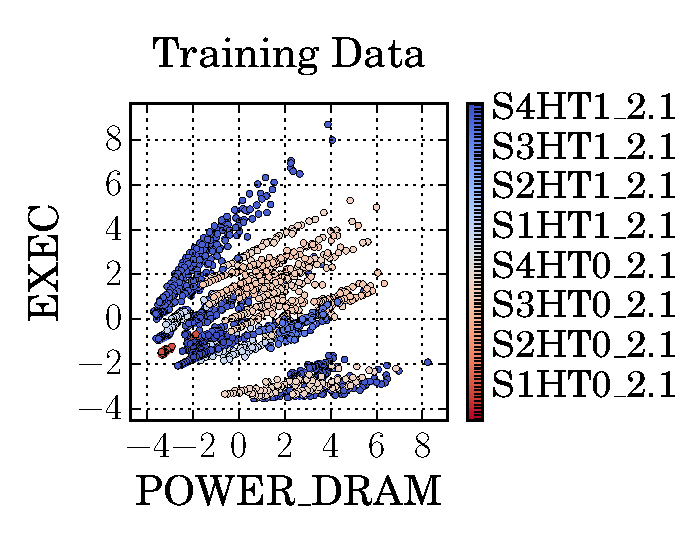
\includegraphics[]{figures/training_space_noclassifier.pdf}
  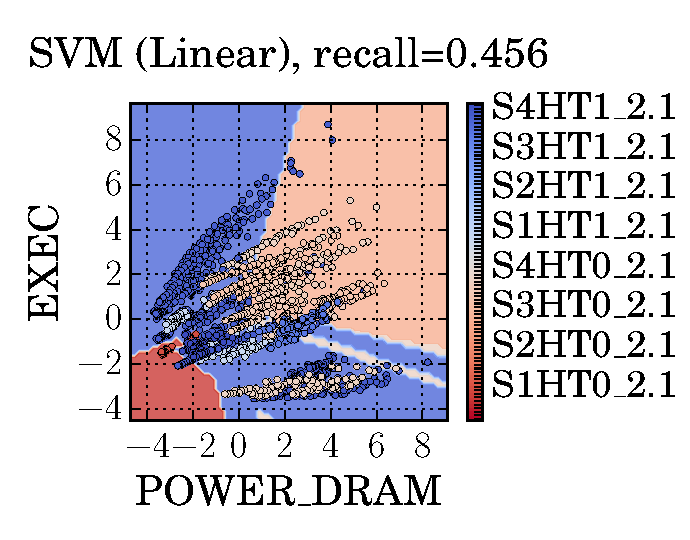
\includegraphics[]{figures/training_space_svm_kern_lin.pdf}
  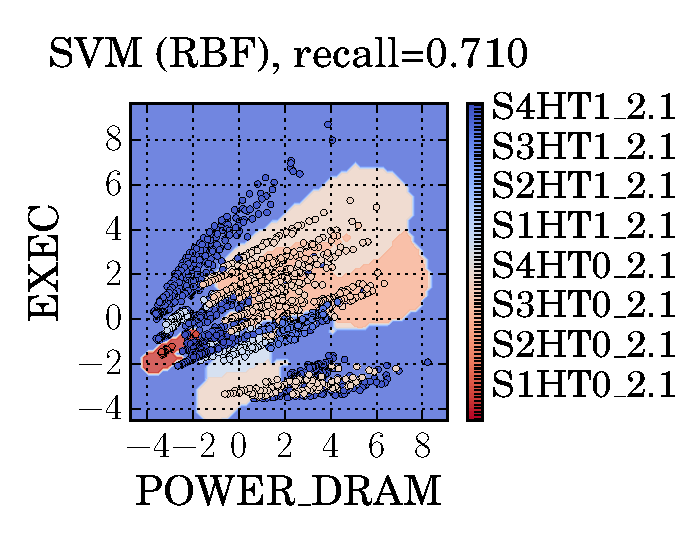
\includegraphics[]{figures/training_space_svm.pdf}
  \captionof{figure}{Training data features; SVM (Linear) and SVM (RBF) predictions.}
  \label{fig:classifier-training}
\PAD
}

Training data is collected from characterizations of smaller HPC applications, \eg NAS Parallel Benchmarks, Co-design benchmarks, and proxy applications.
Our evaluation system produces 88 data points for each training application (1 per configuration)---all 88 are labeled using the most energy-efficient configuration for that application.
\textbf{Principal Component Analysis} determines which \textbf{features} are most relevant to energy efficiency---\pc{POWER\_DRAM} and \pc{EXEC} are the most useful.

The feature space is complex---no obvious mapping for determining the most energy-efficient state exists, even considering only the top two performance counters.
Simple classifiers are not up to the task, \eg a Linear Support Vector Machine (SVM) recalls less than half of the training data.
A SVM with a RBF kernel performs better.


% \vspace{-1cm}
\section*{Evaluation}

We evaluate our approach on a quad-socket (160-logical-core) system with Intel Xeon E7-8870 processors and 512 GB of DRAM using four HPC bioinformatic applications, which are often run on such large systems.
We test five of the most promising classifiers: Extra Trees (ET), Gradient Boosting (GB), K-Nearest Neighbors (KNN), Multi-layer Perceptron (MLP), and a Support Vector Machine (SVM) with a RBF kernel.

{
\PAD
\PAD
\centering
  \begin{tikzpicture}
\definecolor{s1}{RGB}{228, 26, 28}
\definecolor{s2}{RGB}{55, 126, 184}
\definecolor{s3}{RGB}{77, 175, 74}
\definecolor{s4}{RGB}{152, 78, 163}
\definecolor{s5}{RGB}{255, 127, 0}

\begin{groupplot}[
    group style={
        group name=plots,
        group size=1 by 1,
        xlabels at=edge bottom,
        xticklabels at=edge bottom,
        vertical sep=5pt
    },
% axis x line* = bottom,
xlabel near ticks,
major x tick style = transparent,
xlabel={},
height=8cm,
width=0.8\columnwidth,
xmin=0.5,
xmax=4.5,
enlargelimits=false,
tick align = outside,
tick style={white},
ylabel style={align=center},
ytick=\empty,
ymin=0.6,
ymax=1.05,
ytick={0,0.2,0.4,0.6,0.8,1.0,1.2},
yticklabels={0.0,0.2,0.4,0.6,0.8,1.0,1.2},
legend cell align=left, 
legend style={ column sep=1ex },
ymajorgrids,
grid style={dashed},
]

\nextgroupplot[ylabel={Energy \\ (Normalized)},
ybar=\pgflinewidth,
legend entries = {ET,GB,KNN,MLP,SVM,Oracle},
legend style={draw=none,legend columns=6,at={(.5,1.25)},anchor=north},
bar width=18pt,
ylabel shift={0mm},
xticklabel shift={0pt},
x tick label style={rotate=35, anchor=east},
xtick={1,2,3,4,5,6,7},
xticklabels={
{HipMer},
{IDBA},
{Megahit},
{metaSPAdes},
},
execute at end plot={
% "Race":
\draw[thin, dashed] (axis cs:\pgfkeysvalueof{/pgfplots/xmin},1) -- (axis cs:\pgfkeysvalueof{/pgfplots/xmax},1);
% "Best static DVFS":
% \draw[thick, dotted] (axis cs:\pgfkeysvalueof{/pgfplots/xmin},0.765646972) -- (axis cs:\pgfkeysvalueof{/pgfplots/xmax},0.765646972);
% hack to reset column line style (ghostscript seems to use last formatting as line style, e.g. dashed or dotted instead of solid)
\draw[thin, solid] (axis cs:\pgfkeysvalueof{/pgfplots/xmin},\pgfkeysvalueof{/pgfplots/ymin}) -- (axis cs:\pgfkeysvalueof{/pgfplots/xmax},\pgfkeysvalueof{/pgfplots/ymin});
},
]
\addplot table[x index=0,y index=2, col sep=tab] {img/compare_apps_pca4.txt};
\addplot table[x index=0,y index=3, col sep=tab] {img/compare_apps_pca4.txt};
\addplot table[x index=0,y index=4, col sep=tab] {img/compare_apps_pca4.txt};
\addplot table[x index=0,y index=5, col sep=tab] {img/compare_apps_pca4.txt};
\addplot table[x index=0,y index=6, col sep=tab] {img/compare_apps_pca4.txt};
\addplot table[x index=0,y index=7, col sep=tab] {img/compare_apps_pca4.txt};

\end{groupplot}

\end{tikzpicture}
  \captionof{figure}{Average application energy consumption using four performance counters at 5 second prediction intervals (lower is better).}
  \label{fig:compare-apps-pca4}
\PAD
}

\figref{compare-apps-pca4} demonstrates results for each application, normalized to the \emph{race-to-idle} heuristic (dashed line) for each.
On average across all four applications, energy consumption is reduced by 19.3\%.

{
\PAD
\PAD
\centering
  \begin{tikzpicture}
\begin{centering}

\definecolor{s1}{RGB}{228, 26, 28}
\definecolor{s2}{RGB}{55, 126, 184}
\definecolor{s3}{RGB}{77, 175, 74}
\definecolor{s4}{RGB}{152, 78, 163}
\definecolor{s5}{RGB}{255, 127, 0}

\begin{groupplot}[
    group style={
        group name=plots,
        group size=1 by 1,
        xlabels at=edge bottom,
        xticklabels at=edge bottom,
        vertical sep=5pt
    },
height=8cm,
width=0.8\columnwidth,
xmajorgrids,
ymajorgrids,
grid style={dashed},
xmin=0,
xmax=3465,
xtick={0,500,1000,1500,2000,2500,3000,3500},
ymin=0,
ymax=1.05,
ytick={0,0.2,0.4,0.6,0.8,1.0},
yticklabels={0,0.2,0.4,0.6,0.8,1.0},
yticklabel pos=left,
enlargelimits=false,
tick align = outside,
tick style={white},
xticklabel shift={-5pt},
yticklabel shift={-5pt},
ylabel shift={-2pt},
ylabel style={align=center},
unbounded coords=jump,
legend cell align=left, 
legend style={ column sep=1ex },
]

\nextgroupplot[ylabel={},
% yticklabel style={font=\footnotesize},
xlabel={$time$ [seconds]},
xlabel near ticks,
xticklabels={0,500,1000,1500,2000,2500,3000,3500},
% xticklabel style={font=\footnotesize},
legend entries={{Power},{EE},{Cumulative Energy}},
legend style={draw=none,at={(0.5,1.25)},anchor=north,legend columns=4,line width=5pt},
]
\addplot[very thick, solid, color=s2] table[x index=0,y index=1,col sep=comma] {img/ts_hipmer/ts_hipmer_2101000_pca4.csv};
\addplot[very thick, solid, color=s3] table[x index=0,y index=2,col sep=comma] {img/ts_hipmer/ts_hipmer_2101000_pca4.csv};
\addplot[very thick, solid, color=s1] table[x index=0,y index=3,col sep=comma] {img/ts_hipmer/ts_hipmer_2101000_pca4.csv};
\addplot[thin, solid, black] coordinates {(2206,0) (2206, 2)};

\end{groupplot}
\end{centering}

\end{tikzpicture}
  \captionof{figure}{HipMer in naive static \emph{race-to-idle} heuristic.}
  \label{fig:ts-hipmer-dvfs}
\PAD
}

{
\PAD
\centering
  \begin{tikzpicture}
\begin{centering}

\definecolor{s1}{RGB}{228, 26, 28}
\definecolor{s2}{RGB}{55, 126, 184}
\definecolor{s3}{RGB}{77, 175, 74}
\definecolor{s4}{RGB}{152, 78, 163}
\definecolor{s5}{RGB}{255, 127, 0}

\begin{groupplot}[
    group style={
        group name=plots,
        group size=1 by 1,
        xlabels at=edge bottom,
        xticklabels at=edge bottom,
        vertical sep=5pt
    },
height=8cm,
width=0.8\columnwidth,
xmajorgrids,
ymajorgrids,
grid style={dashed},
xmin=0,
xmax=3465,
xtick={0,500,1000,1500,2000,2500,3000,3500},
ymin=0,
ymax=1.05,
ytick={0,0.2,0.4,0.6,0.8,1.0},
yticklabels={0,0.2,0.4,0.6,0.8,1.0},
yticklabel pos=left,
enlargelimits=false,
tick align = outside,
tick style={white},
xticklabel shift={-5pt},
yticklabel shift={-5pt},
ylabel shift={-2pt},
ylabel style={align=center},
unbounded coords=jump,
legend cell align=left, 
legend style={ column sep=1ex },
]

\nextgroupplot[ylabel={},
% yticklabel style={font=\footnotesize},
xlabel={$time$ [seconds]},
xlabel near ticks,
xticklabels={0,500,1000,1500,2000,2500,3000,3500},
% xticklabel style={font=\footnotesize},
legend entries={{Power},{EE},{Cumulative Energy}},
legend style={draw=none,at={(0.5,1.25)},anchor=north,legend columns=4,line width=5pt},
]
\addplot[very thick, solid, color=s2] table[x index=0,y index=1,col sep=comma] {img/ts_hipmer/ts_hipmer_et_pca4.csv};
\addplot[very thick, solid, color=s3] table[x index=0,y index=2,col sep=comma] {img/ts_hipmer/ts_hipmer_et_pca4.csv};
\addplot[very thick, solid, color=s1] table[x index=0,y index=3,col sep=comma] {img/ts_hipmer/ts_hipmer_et_pca4.csv};
\addplot[thin, solid, black] coordinates {(3465,0) (3465, 2)};

\end{groupplot}
\end{centering}

\end{tikzpicture}
  \captionof{figure}{HipMer with ET classifier at 5 second intervals.}
  \label{fig:ts-hipmer-all-et}
\PAD
}

To demonstrate how energy savings are achieved, \figref{ts-hipmer-dvfs} runs HipMer in the \emph{race-to-idle} heuristic, and although the runtime is short, the high power also results in poor energy consumption.
In contrast, \figref{ts-hipmer-all-et} demonstrates running with the ET classifier---the execution takes longer, but the significantly lower power results in nearly 20\% less energy consumption in total, despite the increase in runtime.


% \vfill\null
% \columnbreak

%------------------------------------------------

%\subsection*{Mathematical Section}



%----------------------------------------------------------------------------------------
% RESULTS 
%----------------------------------------------------------------------------------------




%----------------------------------------------------------------------------------------
%	CONCLUSIONS
%----------------------------------------------------------------------------------------
\color{SaddleBrown} % SaddleBrown color for the conclusions to make them stand out

\section*{Conclusions}

Not only does our approach reduce the cost per scientific insight, but scaling this improvement to an over-provisioned, power-constrained cluster could increase total cluster throughput.
By trading performance for power savings, maximizing energy efficiency could \emph{increase the total throughput of a hardware over-provisioned system by up to 40\%.}


\color{DarkSlateGray} % Set the color back to DarkSlateGray for the rest of the content

%----------------------------------------------------------------------------------------
%	FORTHCOMING RESEARCH
%----------------------------------------------------------------------------------------

%\section*{Forthcoming Research}



 %----------------------------------------------------------------------------------------
%	REFERENCES
%----------------------------------------------------------------------------------------

% \printbibliography
%\nocite{*} % Print all references regardless of whether they were cited in the poster or not
%\bibliographystyle{plain} % Plain referencing style
%\bibliography{seec}

%----------------------------------------------------------------------------------------
%	ACKNOWLEDGEMENTS
%----------------------------------------------------------------------------------------

% \vspace{-1cm}
\section*{Acknowledgements}

\small
The effort on this project is funded by the U.S. Government under the DARPA BRASS program, by the Dept. of Energy under DOE DE-AC02-06CH11357, by the NSF under CCF 1439156, and by a DOE Early Career Award.\\
Part of this research was conducted while Connor Imes was a Computing Sciences Summer Student at Lawrence Berkeley National Laboratory.

%----------------------------------------------------------------------------------------

\end{multicols}

% \begin{minipage}[b]{\linewidth}
\begin{center}
\vspace{0.5cm}
\Large \texttt{https://people.cs.uchicago.edu/{\raise.17ex\hbox{$\scriptstyle\mathtt{\sim}$}}ckimes/}
% \Large \texttt{http://poet.cs.uchicago.edu/}~~~~~~$\vert$~~~~~~\texttt{http://github.com/energymon/}~~~~~~$\vert$~~~~~~\texttt{http://github.com/powercap/}
\end{center}
% \end{minipage}

\end{document}